\documentclass[border=2pt]{standalone}
\usepackage{tikz}
\usetikzlibrary{trees}

\tikzset{
  term/.style={draw,circle,minimum size=8mm,inner sep=1pt},
  derivative/.style={draw,rounded corners=2pt,inner sep=2pt}
}

\begin{document}
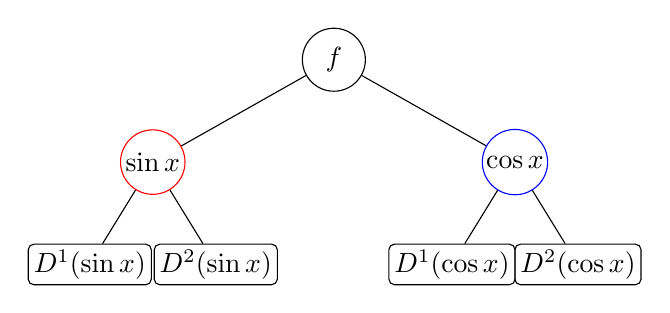
\begin{tikzpicture}[
  grow=down,
  level distance=13mm,
  level 1/.style={sibling distance=46mm},
  level 2/.style={sibling distance=16mm}
]
  \node[term] {$f$}
    child foreach \op/\tone in {\sin/red,\cos/blue} {
      node[term,draw=\tone] {$\op x$}
      child foreach \order in {1,2}
        {node[derivative] {$D^{\order}(\op x)$}}
    };
\end{tikzpicture}
\end{document}
